\documentclass{beamer}
%
% Choose how your presentation looks.
%
% For more themes, color themes and font themes, see:
% http://deic.uab.es/~iblanes/beamer_gallery/index_by_theme.html
%
\mode<presentation>
{
  \usetheme{default}      % or try Darmstadt, Madrid, Warsaw, ...
  \usecolortheme{default} % or try albatross, beaver, crane, ...
  \usefonttheme{default}  % or try serif, structurebold, ...
  \setbeamertemplate{navigation symbols}{}
  \setbeamertemplate{caption}[numbered]
} 

\usepackage[english]{babel}
\usepackage[utf8]{inputenc}
\usepackage[T1]{fontenc}

\usepackage{algpseudocode}

\usepackage[numbers,sort&compress]{natbib}

\title{Attacking the Vigenere Cipher\\with Pattern Theory}
\author{Daniel Yao}
\institute{Johns Hopkins University}
\date{25 April 2025}

%%%

\begin{document}

\begin{frame}

\titlepage

\end{frame}

%%

\begin{frame}{Introduction}

\begin{block}{Example}
\end{block}

\vspace{-12pt}

\begin{center}
\begin{tabular}{c|ccccc}
  plaintext & z & e & b & r & a \\
  \hline
  key & \textcolor{blue}{b} & \textcolor{blue}{a} & b & a & b \\
  \hline
  ciphertext & a & e & c & r & b \\
\end{tabular}
\end{center}

\begin{block}{Table}
\end{block}

\vspace{-12pt}

\begin{center}
\begin{tabular}{c|*{13}{c}}
 & a & b & c & d & e & f & g & h & i & j & k & l & m \\
\hline
\textcolor{blue}{a} & a & b & c & d & e & f & g & h & i & j & k & l & m \\
\textcolor{blue}{b} & b & c & d & e & f & g & h & i & j & k & l & m & n \\
\end{tabular}
\end{center}

\begin{center}
\begin{tabular}{c|*{13}{c}}
 & n & o & p & q & r & s & t & u & v & w & x & y & z \\
\hline
\textcolor{blue}{a} & n & o & p & q & r & s & t & u & v & w & x & y & z \\
\textcolor{blue}{b} & o & p & q & r & s & t & u & v & w & x & y & z & a \\
\end{tabular}
\end{center}

\end{frame}

%%

\begin{frame}{Introduction}

\begin{block}{Vigenere Cipher \cite{vigenere1586}}
\begin{itemize}
\item A Vigenere cipher with key $k = (k_{1}, \ldots, k_{K}$) is a map $f: A^{N} \to A^{N}$ where for $i = 1, \ldots, N$,
$$f_{i}(x_{i}) = (x_{i} + k_{i \text{ mod } K}) \text{ mod } |A|.$$
\item To decipher, we need the inverse function 
$$f^{-1}_{i}(y_{i}) = (y_{i} - k_{i \text{ mod } K}) \text{ mod } |A|.$$
\end{itemize}
\end{block}

\begin{block}{Example}
\end{block}

\vspace{-12pt}

\begin{center}
\begin{tabular}{c|ccccc}
  plaintext & z & e & b & r & a \\
  \hline
  key & \textcolor{blue}{b} & \textcolor{blue}{a} & b & a & b \\
  \hline
  ciphertext & a & e & c & r & b \\
\end{tabular}
\end{center}

\end{frame}

%%

\begin{frame}{Introduction}

\begin{block}{Decipher with key length $K=3$}
\begin{itemize}
\item \textcolor{red}{iubwbu ujeagppehaqfademkegbiubwbu ujeagppehaqfakndteewljvy}
\end{itemize}
\end{block}

\end{frame}

%%

\begin{frame}{Introduction}

\begin{block}{Decipher with key length $K=3$}
\begin{itemize}
\item \textcolor{red}{iubwbu ujeagppehaqfademkegbiubwbu ujeagppehaqfakndteewljvy}
\item \textcolor{red}{iubwbu }\textcolor{blue}{uje}\textcolor{red}{agppehaqfademkegbiubwbu }\textcolor{blue}{uje}\textcolor{red}{agppehaqfakndteewljvy}
\end{itemize}
\end{block}

\end{frame}
  
%%

\begin{frame}{Introduction}

\begin{block}{Decipher with key length $K=3$}
\begin{itemize}
\item \textcolor{red}{iubwbu ujeagppehaqfademkegbiubwbu ujeagppehaqfakndteewljvy}
\item \textcolor{red}{iubwbu }\textcolor{blue}{uje}\textcolor{red}{agppehaqfademkegbiubwbu }\textcolor{blue}{uje}\textcolor{red}{agppehaqfakndteewljvy}
\item it was \textcolor{blue}{the} epoch of belief it was \textcolor{blue}{the} epoch of incredulity
\end{itemize}
\end{block}

\end{frame}

%%

\begin{frame}{Introduction}

\begin{block}{Decipher with key length $K=3$}
\begin{itemize}
\item \textcolor{red}{iubwbu ujeagppehaqfademkegbiubwbu ujeagppehaqfakndteewljvy}
\item \textcolor{red}{iubwbu }\textcolor{blue}{uje}\textcolor{red}{agppehaqfademkegbiubwbu }\textcolor{blue}{uje}\textcolor{red}{agppehaqfakndteewljvy}
\item it was \textcolor{blue}{the} epoch of belief it was \textcolor{blue}{the} epoch of incredulity
\end{itemize}
\end{block}

\begin{block}{Solution}
\begin{itemize}
\item \textcolor{blue}{abc}
\end{itemize}
\end{block}

\end{frame}

%%

\begin{frame}{Introduction}

\begin{block}{Language Model \cite{menon2020pattern}}
\begin{itemize}
\item English is a stationary ergodic stochastic process with state space (alphabet)
$$A = \{a, \ldots, z, \_\}.$$
\item The \textit{character $2$-gram model} is that English is a Markov chain $X_{1}, X_{2}, \ldots$ with state space $A$ and transition matrix 
$$Q^{(2)}(x_{1}, x_{0}) = P(X_{1} = x_{1} \mid X_{0} = x_{0}).$$
\end{itemize}
\end{block}

\begin{block}{Example}
\begin{itemize}
\item If $n = 2$, then $(X_{0}, X_{1}, X_{2}) = (\text{t}, \text{h}, \text{e})$ has probability 
\begin{align*}
P(\text{t}, \text{h}, \text{e}) &= P(\text{t}) P(\text{h} \mid \text{t}) P(\text{e} \mid \text{h}) \\
                              &= 0.07498(0.2828)(0.4321).
\end{align*}
\end{itemize}
\end{block}

\end{frame}

%%

\begin{frame}{Introduction}

\begin{center} 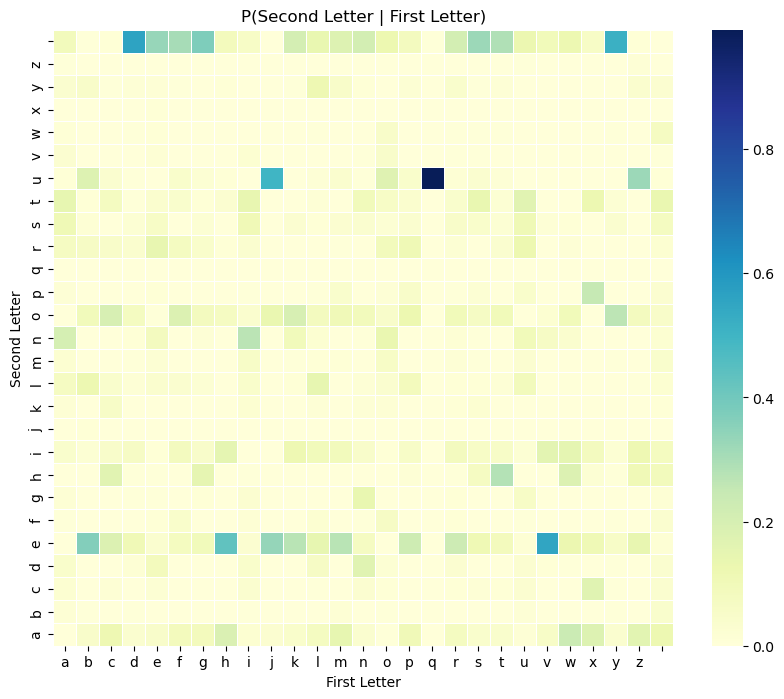
\includegraphics[width=3.5in]{images/heatmap.png} \end{center}

\end{frame}

%%

\begin{frame}{Methods}

\begin{block}{Maximum Likelihood Estimation}
\begin{itemize}
\item Given an encoded text $(y_{0}, \ldots, y_{N})$ and key length $K$, we want to find the decoded text $f^{-1}(y_{0}, \ldots, y_{N})$.
\item The posterior probability that $f$ is the true cipher is
$$P(f \mid y) = \frac{\textcolor{blue}{P(y \mid f)}P(f)}{P(y)} \propto \textcolor{blue}{L(f)}.$$
\item The \textit{likelihood function} is 
\begin{align*}
{L(f)} &= P(f_{0}^{-1}(y_{0}), \ldots, f_{N}^{-1}(y_{N})) \\
      &= Q^{(1)}(f_{0}^{-1}(y_{0})) \prod_{i=1}^{N} Q^{(2)}(f_{i-1}^{-1}(y_{i-1}), f_{i}^{-1}(y_{i})).
\end{align*}
\item The \textit{objective} is to find the best cipher
$$f^{*} = \arg\max L(f).$$
\end{itemize}
\end{block}

\end{frame}

%%

\begin{frame}{Methods}

\begin{block}{Gibbs Sampling \cite{menon2020pattern}}
\begin{itemize}
\item The number of ciphers is $|A|^{K}$, so the posterior is intractable.
\item Turns out, we can use a Gibbs sampling, a \textit{Markov chain Monte Carlo} method that samples from the likelihood distribution $L(f)$.
\item We want to construct a Markov chain on the set of ciphers that has the (limiting) \textit{stationary distribution} $p_{\beta}(f)$ where 
$$\arg\max p_{\beta}(f) = \arg\max L(f).$$
\item The inverse temperature $\beta$ controls the amount of exploration.
\end{itemize}
\end{block}

\end{frame}

%%

\begin{frame}{Methods}

\begin{block}{Experiment \cite{bird2009nlp} \cite{dickens1859tale} \cite{dostoevsky1866crime}}
\begin{itemize}
\item Corpus: \textit{Crime and Punishment} by Fyodor Dostoevsky
\item Text: "It was the best of times, it was the worst of times..." ($N = 592$) from \textit{A Tale of Two Cities} by Charles Dickens
\item Key lengths: $K = 592, 296, 197, 148, 118, \ldots, 1$.
\item Hyperparameters: $M = 10^{5}$, $\beta = 0.5$.
\end{itemize}
\end{block}

\end{frame}

%%

\begin{frame}{Results}

\begin{block}{$K=592$}
\begin{itemize}
\item \textcolor{red}{rn} \textcolor{red}{cte} \textcolor{red}{om\_ghycuf}o\textcolor{red}{t} \textcolor{red}{ad\_ali\_hothtsicute\_d}s\textcolor{red}{e\_u\_llno t}
\end{itemize}
\end{block}

\begin{block}{$K=296$}
\begin{itemize}
\item \textcolor{red}{er} was\textcolor{red}{sap\_o\_}e\textcolor{red}{rhtast\_}i\textcolor{red}{rge} i\textcolor{red}{n} \textcolor{red}{eedu}the\textcolor{red}{do\_na}t \textcolor{red}{g\_hagrki}
\end{itemize}
\end{block}

\begin{block}{$K=197$}
\begin{itemize}
\item it wa\textcolor{red}{t} the bes\textcolor{red}{ee\_}f\textcolor{red}{i\_w}i\textcolor{red}{d}e\textcolor{red}{n} \textcolor{red}{wan\_wi}the \textcolor{red}{dr\_}st \textcolor{red}{pe} t\textcolor{red}{a\_ar}
\end{itemize}
\end{block}

\begin{block}{$K=148$}
\begin{itemize}
\item it was the best of t\textcolor{red}{e\_r}s it was \textcolor{red}{e}he worst\textcolor{red}{t}of t\textcolor{red}{\_y}es
\end{itemize}
\end{block}

\begin{block}{$K=118$}
\begin{itemize}
\item it was the best of times it was the \textcolor{red}{p\_r}st of times
\end{itemize}
\end{block}

\end{frame}

%%

\begin{frame}{Results}

\begin{center}
\begin{tabular}{ccccc}
\hline
$K$ & $N/K$ & Count & Accuracy & Run Time (s) \\
\hline
592 & $N/1$ & 49   & 0.0828 & 598 \\
296 & $N/2$ & 130  & 0.2196 & 360 \\
197 & $N/3$ & 232  & 0.3919 & 303 \\
148 & $N/4$ & 480  & 0.8108 & 258 \\
118 & $N/5$ & 547  & 0.9240 & 190 \\
98  & $N/6$ & 586  & 0.9899 & 119 \\
84  & $N/7$ & 592  & 1.0000 & 76  \\
$\vdots$ & $\vdots$ & $\vdots$ & $\vdots$ & $\vdots$ \\
10  & $N/59$  & 592 & 1.0000 & 1   \\
$\vdots$ & $\vdots$ & $\vdots$ & $\vdots$ & $\vdots$ \\
1   & $N/592$ & 592 & 1.0000 & 0   \\
\hline
\end{tabular}
\end{center}

\end{frame}

%%

\begin{frame}{Results}

\begin{center} 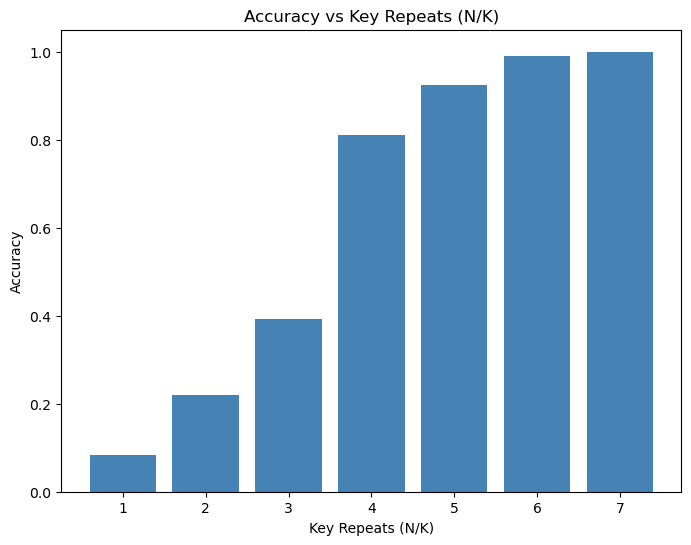
\includegraphics[width=4in]{images/experiment.png} \end{center}

\end{frame}

%%

\begin{frame}{Conclusion}

\begin{block}{Conclusion}
\begin{itemize}
\item Accuracy increases with number of key repeats.
\item With $N/K = 4$ key repeats, Gibbs sampling yields human-readable text.
\end{itemize}
\end{block}

\begin{block}{Next Steps}
\begin{itemize}
\item Try longer/shorter texts.
\item Try stronger language model with longer $n$-grams.
\item Try more complex ciphers (e.g., running key cipher).
\end{itemize}
\end{block}

\end{frame}

%%

\begin{frame}{References}

\bibliographystyle{apalike}
\bibliography{refs}

\end{frame}

%%

% \begin{frame}{Appendix}

% \begin{block}{Running Key Cipher}
% \begin{itemize}
% \item If $n = N$, then the Vigenere cipher is a running key cipher.
% \item If $k$ has no structure, then the running key cipher is unbreakable.
% \item However, $k$ is often another text, i.e., natural language.
% \end{itemize}
% \end{block}

% \begin{block}{Posterior Odds}
% \begin{itemize}
% \item Lorem ipsum dolor sit amet, consectetur adipiscing elit. Donec a diam lectus. Sed sit amet ipsum mauris.
% \end{itemize}
% \end{block}

% \end{frame}

%%

% \begin{frame}{Introduction}

% \begin{block}{Decipher with 5-letter key}
% \begin{itemize}
% \item \textcolor{red}{tzwr omhlkxt fdwpjsooxnlcaybsslu nrfvlghlxyox dlxafklfvyhciraaxagcrgjksjlp}
% \end{itemize}
% \end{block}

% \begin{block}{todsavg ($n=10^{2}$)}
% \begin{itemize}
% \item al\textcolor{red}{t} \textcolor{red}{\_ug}py\textcolor{red}{h}f\textcolor{red}{tf\_}li\textcolor{red}{m}s\textcolor{red}{sui}e \textcolor{red}{i}l\textcolor{red}{adw} e\textcolor{red}{i}c\textcolor{red}{\_tl}nh\textcolor{red}{i}p\textcolor{red}{hrr}fa\textcolor{red}{u}i\textcolor{red}{drr}is\textcolor{red}{h}u\textcolor{red}{fas}pp
% \textcolor{red}{f} \textcolor{red}{agr}it\textcolor{red}{\_} 
% \textcolor{red}{gpe} w\textcolor{red}{i}y
% \end{itemize}
% \end{block}

% \end{frame}

%%

% \begin{frame}{Introduction}

% \begin{block}{Decipher with 5-letter key}
% \begin{itemize}
% \item \textcolor{red}{tzwr omhlkxt fdwpjsooxnlcaybsslu nrfvlghlxyox dlxafklfvyhciraaxagcrgjksjlp}
% \end{itemize}
% \end{block}

% \begin{block}{tolstvg ($n=10^{3}$)}
% \begin{itemize}
% \item al\textcolor{red}{t} \textcolor{red}{\_ug}py\textcolor{red}{h}f\textcolor{red}{tf\_}li\textcolor{red}{m}s\textcolor{red}{sui}e \textcolor{red}{i}l\textcolor{red}{adw} e\textcolor{red}{i}c\textcolor{red}{\_tl}nh\textcolor{red}{i}p\textcolor{red}{hrr}fa\textcolor{red}{u}i\textcolor{red}{drr}is\textcolor{red}{h}u\textcolor{red}{fas}pp
% \textcolor{red}{f} \textcolor{red}{agr}it\textcolor{red}{\_} 
% \textcolor{red}{gpe} w\textcolor{red}{i}y
% \item all h\textcolor{red}{ug}py fa\textcolor{red}{f\_}lies \textcolor{red}{ui}e ali\textcolor{red}{dw} each\textcolor{red}{tl}nhapp\textcolor{red}{rr}famil\textcolor{red}{rr}is un\textcolor{red}{as}ppy i\textcolor{red}{gr}its o\textcolor{red}{pe} way
% \end{itemize}
% \end{block}

% \end{frame}

%%

% \begin{frame}{Introduction}

% \begin{block}{Decipher with 5-letter key}
% \begin{itemize}
% \item \textcolor{red}{tzwr omhlkxt fdwpjsooxnlcaybsslu nrfvlghlxyox dlxafklfvyhciraaxagcrgjksjlp}
% \end{itemize}
% \end{block}

% \begin{block}{tolstoy ($n=10^{4}$)}
% \begin{itemize}
% \item al\textcolor{red}{t} \textcolor{red}{\_ug}py\textcolor{red}{h}f\textcolor{red}{tf\_}li\textcolor{red}{m}s\textcolor{red}{sui}e \textcolor{red}{i}l\textcolor{red}{adw} e\textcolor{red}{i}c\textcolor{red}{\_tl}nh\textcolor{red}{i}p\textcolor{red}{hrr}fa\textcolor{red}{u}i\textcolor{red}{drr}is\textcolor{red}{h}u\textcolor{red}{fas}pp
% \textcolor{red}{f} \textcolor{red}{agr}it\textcolor{red}{\_} 
% \textcolor{red}{gpe} w\textcolor{red}{i}y
% \item all h\textcolor{red}{ug}py fa\textcolor{red}{f\_}lies \textcolor{red}{ui}e ali\textcolor{red}{dw} each\textcolor{red}{tl}nhapp\textcolor{red}{rr}famil\textcolor{red}{rr}is un\textcolor{red}{as}ppy i\textcolor{red}{gr}its o\textcolor{red}{pe} way
% \item all happy families are alike each unhappy family is unhappy in its own way
% \end{itemize}
% \end{block}

% \end{frame}

%%

% \begin{frame}{Introduction}

% \begin{block}{Substitution Cipher}
% \begin{itemize}
% \item A substitution cipher permutation $\sigma: A \to A$ is a map $f: A^{N} \to A^{N}$ where 
% $$f(x_{0}, \ldots, x_{N}) = (\sigma(x_{0}), \ldots, \sigma(x_{N}))$$
% \end{itemize}
% \end{block}

% \end{frame}

%%

% \begin{frame}{Appendix}

% \begin{block}{Reddy and Knight (2012)}
% \begin{itemize}
% \item Lorem ipsum dolor sit amet, consectetur adipiscing elit. Donec a diam lectus. Sed sit amet ipsum mauris.
% \end{itemize}
% \end{block}

% \end{frame}

%%

\begin{frame}{Appendix}

\begin{block}{Gibbs Sampling \cite{menon2020pattern}}
\begin{itemize}
\item Gibbs sampling as a Markov chain Monte Carlo method to sample from the posterior distribution of $\sigma$.
\item The Gibbs distribution with inverse temperature $\beta$ has the pmf 
$$p_{\beta}(x) = \frac{\exp(-\beta E(x))}{Z_{\beta}}$$
where $E$ is the energy function and $Z_{\beta}$ is the partition function (normalization constant).
\item Let $E(\sigma) = -\log L(\sigma)$. We want to find 
\begin{align*}
\arg\max_{\sigma} L(\sigma) &= arg\max_{\sigma} \exp(-\beta E(\sigma)) \\
                          &= \arg\max_{\sigma} p_{\beta}(\sigma).
\end{align*}
\end{itemize}
\end{block}

\end{frame}

%%

\begin{frame}{Appendix}

\begin{block}{Gibbs Sampling \cite{menon2020pattern}}
\end{block}

\vspace{-12pt}

\begin{algorithmic}
\Procedure{MCMC}{$E$, $\text{newPerm}$, $\beta$, $N$}
\State $\sigma \gets \text{id}$, $\sigma^{*} \gets \sigma$
\For{$i = 1$ to $N$}
  \State $\tau \gets \text{newPerm}(\sigma)$
  \If{$E(\tau) < E(\sigma)$ \textbf{or} $\text{unif}(0, 1) < \exp(-\beta \Delta E)$}
    \State $\sigma \gets \tau$
  \EndIf
  \If($E(\sigma) < E(\sigma^{*})$)
    \State $\sigma^{*} \gets \sigma$
  \EndIf
\EndFor
\State \Return $\sigma^{*}$
\EndProcedure
\end{algorithmic}

\end{frame}

\end{document}